\section{性能评测}
\label{sec:eval}

本节给出端到端评估（\S\ref{ssec:e2e-performance}）以及对三项设计原则的实验分析。

\begin{figure*}[tb]
\centering
\begin{subfigure}[b]{0.466\linewidth}
\centering
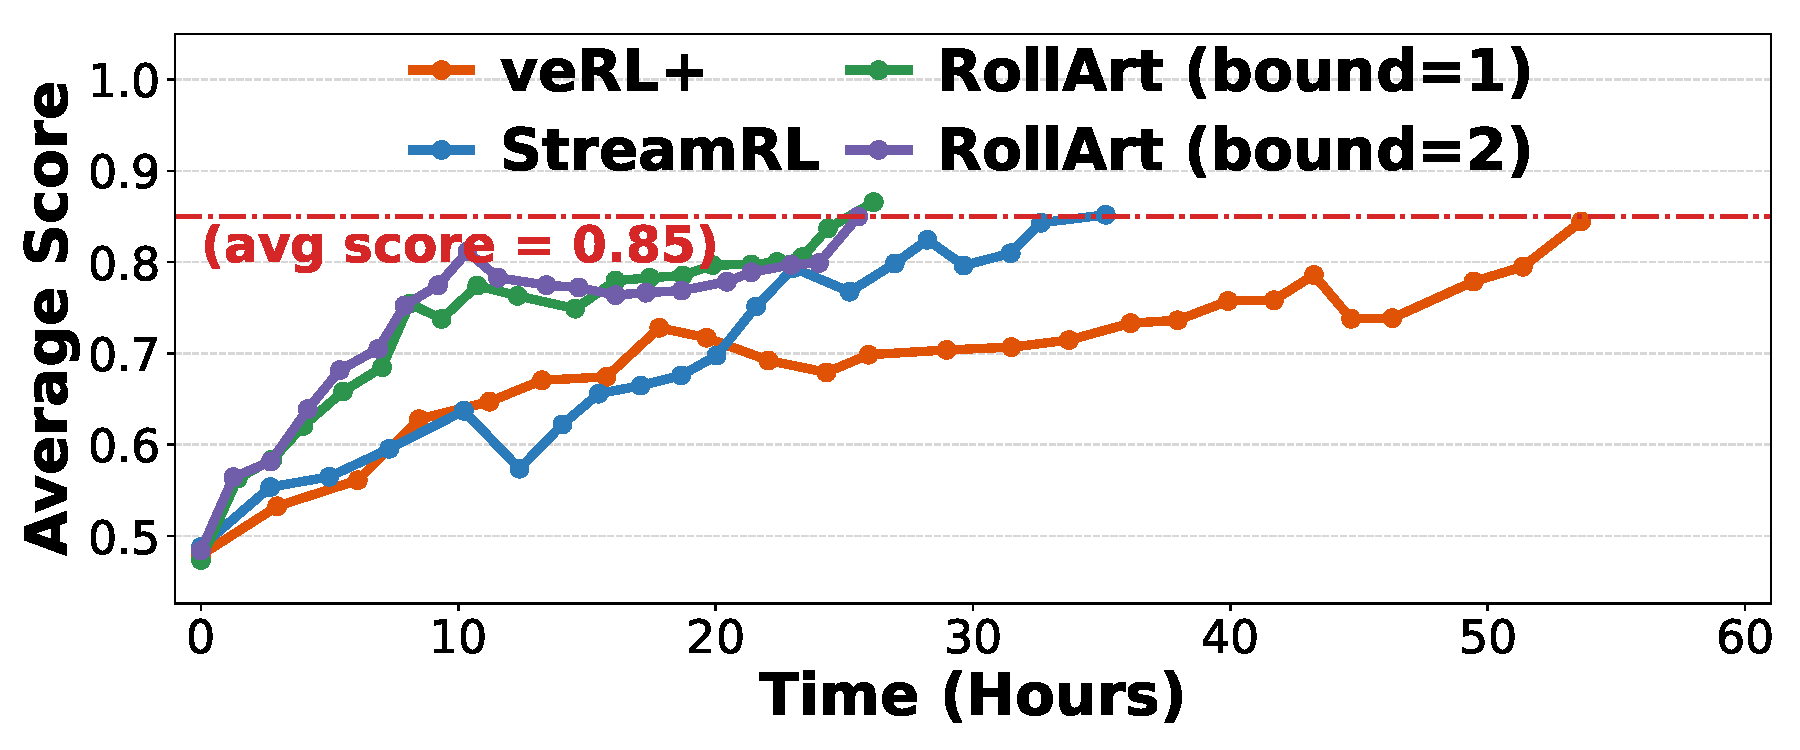
\includegraphics[width=\linewidth]{figs/e2e/score_comparison.pdf}
\caption{达到目标分数所需时间。}
\label{fig:e2e-acc}
\end{subfigure}
\begin{subfigure}[b]{0.31\linewidth}
\centering
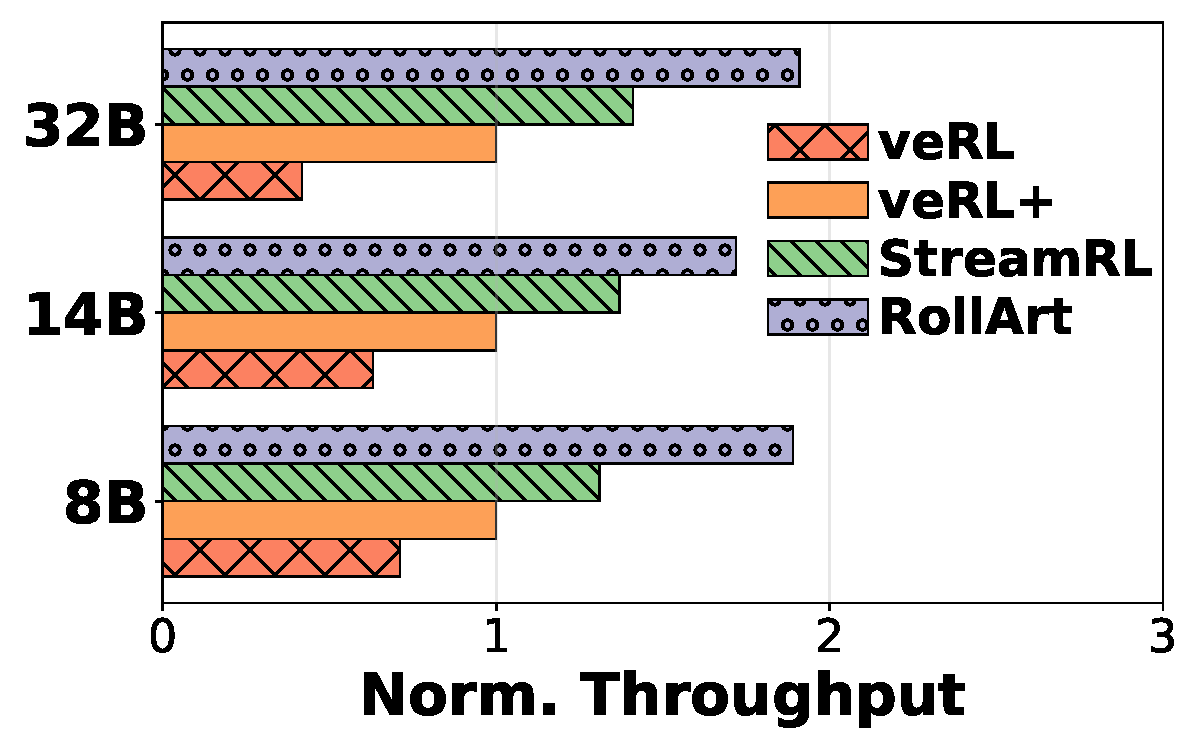
\includegraphics[width=\linewidth]{figs/e2e/modelsize_thr_horizontal.pdf}
\caption{吞吐效率。}
\label{fig:e2e-thr}
\end{subfigure}
\begin{subfigure}[b]{0.214\linewidth}
\centering
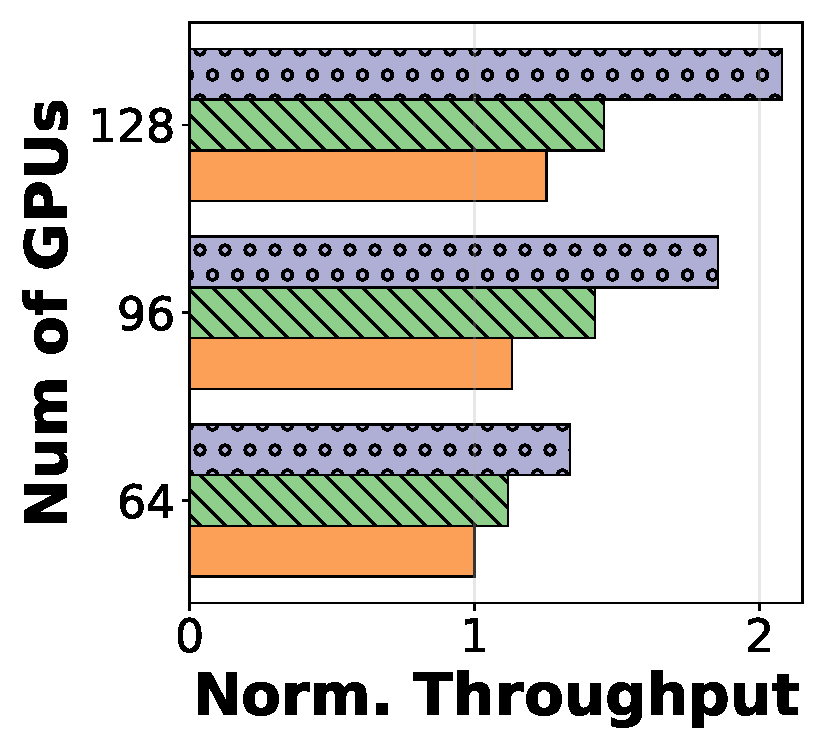
\includegraphics[width=\linewidth]{figs/e2e/modelsize_scaling_horizontal.pdf}
\caption{资源扩展性。}
\label{fig:e2e-thr-scaling}
\end{subfigure}
\caption{(a) Qwen3-32B 的 time-to-score 对比；(b) 不同方法在不同 LLM 上的归一化吞吐；(c) Qwen3-14B 在不同 H800 GPU 数量下的归一化吞吐。}
\label{fig:e2e-combined}
\end{figure*}

\subsection{实验设置}

\noindent\textbf{模型与任务。}
我们在多种 agentic 任务混合数据上训练 Qwen3~\cite{yang2025qwen3technicalreport} 系列模型（8B--32B），全部模型的最大上下文长度设为 32K。由于 \texttt{SWE-bench} 难度较高，仅在 Qwen3-32B 上训练该任务。对于数学任务，我们使用一个 7B 奖励 LLM 来验证推理过程。

\noindent\textbf{训练配置。}
我们采用 GRPO~\cite{he2025deepmath}，训练 batch size 为 512，group size 为 8，各任务采用均匀采样。异步训练中，我们为 training 固定分配 32 张 H800，并将其余 H20/H800 用于 rollout。对于 rollout，Qwen3-8B、14B、32B 的张量并行度分别设为 1、2、4，并对训练并行方式做调优以最大化吞吐。rollout 使用 vLLM 0.8.4，训练使用 Megatron v0.12.2，并开启 prefix caching 与 CUDA graphs。

\noindent\textbf{权重更新引擎。}
集群内权重同步使用 NCCL~\cite{nccl} v2.26.5，跨集群通信使用 Mooncake v0.3.7~\cite{qin2024mooncake}。

\noindent\textbf{硬件。}
\SystemName{}部署在一个 96 卡 H800 集群和一个 32 卡 H20 集群上。集群内部通过 400 Gbps InfiniBand 互联，跨集群通过 200 Gbps 以太网通信。\texttt{SWE-bench} 使用独立 CPU 集群，其余环境使用另一套 CPU 集群。奖励工作者运行在内部 serverless 平台上。除非特别说明，实验默认使用 128 张 GPU。

\noindent\textbf{基线。}
由于现有开源系统不能完整覆盖我们的 agentic 任务集合，我们以 veRL 的同步 RL 实现作为主要基线（\textbf{veRL}），并进一步为其补上异步奖励计算、异步环境交互与 \textit{Reward-as-a-Service}，记为 \textbf{veRL+}。同时，我们还对比了 StreamRL~\cite{StreamRL} 及 one-off training 范式~\cite{deepscaler2025}。

\subsection{端到端收益}
\label{ssec:e2e-performance}
\autoref{fig:e2e-combined} 总结了端到端结果。\SystemName{}在 Qwen3-32B 上显著缩短了达到同等任务分数所需的训练时间，并在不同模型规模上保持较高吞吐效率。实验表明，系统在吞吐与 time-to-score 两个维度上都优于同步式与粗粒度解耦式基线。随着 GPU 数量增加，其扩展曲线仍较平滑，说明硬件亲和映射和异步编排能有效释放更多资源。

\subsection{原则 1：解耦与硬件亲和的收益}
\label{subsec:eval-disaggregated}
我们对比了单体式部署、仅做阶段级解耦，以及进一步加入硬件亲和映射三种配置。结果表明，仅按训练与 rollout 阶段拆分已能带来明显收益，但对 agentic RL 而言，这还不足以充分利用异构集群。当系统进一步根据任务特征将 prefill 主导任务路由到 H800、decode 主导任务路由到 H20 时，吞吐还能继续提升。这一结果验证了原则 1：agentic RL 的异构性不仅存在于阶段之间，也存在于 rollout 内部。

\subsection{原则 2：异步执行的收益}
\label{subsec:eval-async}
我们评估了三种细粒度异步机制：轨迹级环境交互、冗余环境 rollout，以及异步边界控制。结果显示，随着 batch size 增大，轨迹级交互相对于批次级交互的收益从 1.23 倍增长到 2.27 倍，说明异步环境交互可以在大规模时持续保持高吞吐。对于冗余环境 rollout，我们在 Qwen3-8B/32K 上同时改变环境组数与 group size，得到最高 1.62 倍的 rollout 加速，且两项参数的增加均带来正收益。

对于异步边界，我们将其从 1 调到 6，观察不同 LLM 的平均 step time。更大的边界通常降低轨迹因陈旧被中止的概率，因此可进一步减少 step time；但收益很快进入平台区，不同模型的最优值也不相同。综合训练稳定性和最终 time-to-score，\SystemName{}在实践中通常将边界设为 1。

\begin{figure}[tb]
\centering
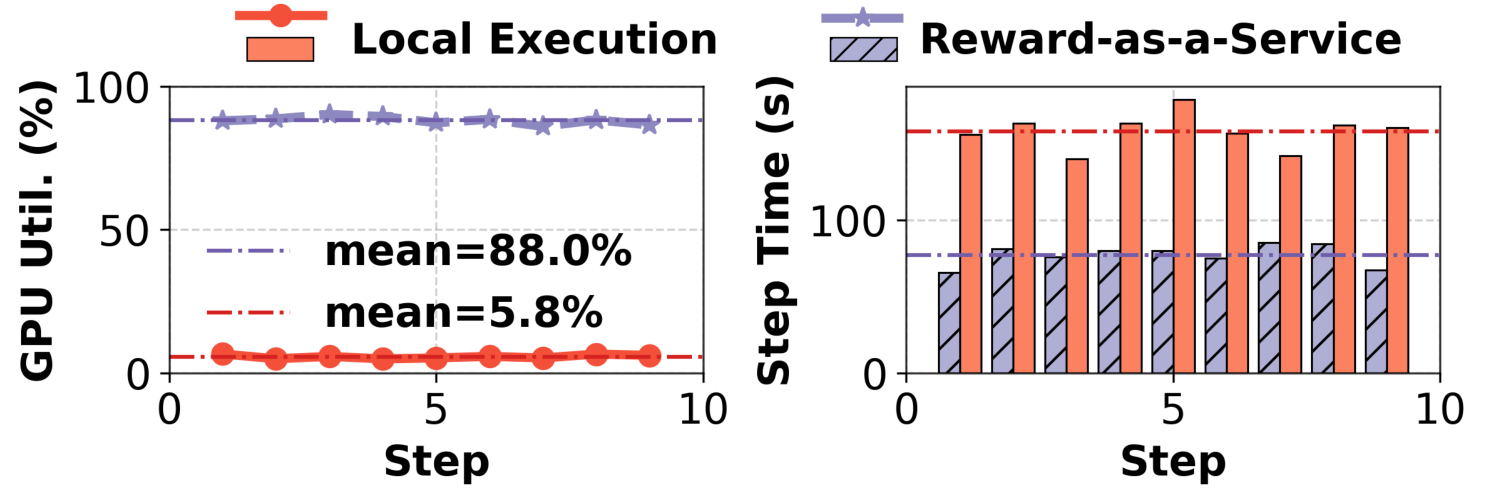
\includegraphics[width=\linewidth]{figs/reward/7B_experiments_comparison.pdf}
\caption{\textbf{[原则 3]}：本地专用 GPU 与 Reward-as-a-Service 的对比。}
\label{fig:reward_comparison_exp}
\end{figure}

\begin{figure*}[tb]
\centering
\begin{subfigure}[b]{0.33\linewidth}
\centering
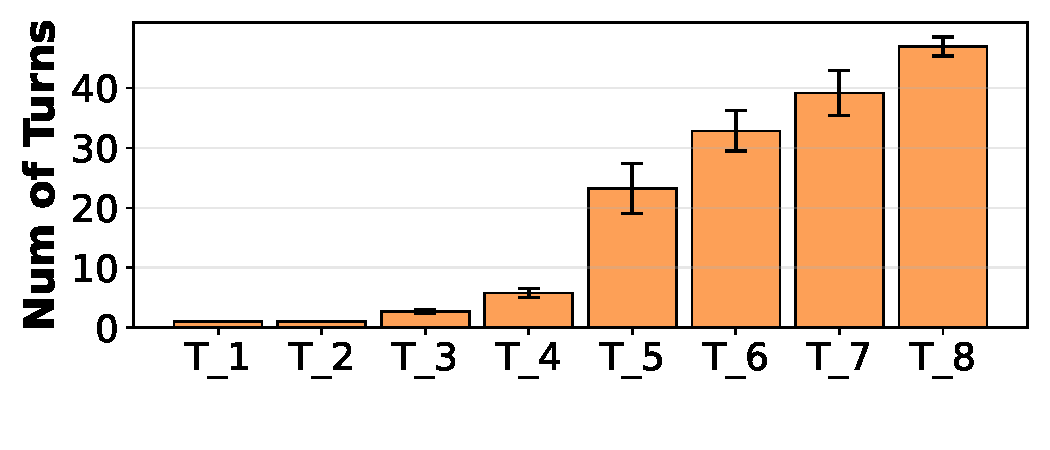
\includegraphics[width=\linewidth]{figs/trace/action.pdf}
\caption{每类任务的平均轮次数。}
\label{fig:action}
\end{subfigure}
\begin{subfigure}[b]{0.33\linewidth}
\centering
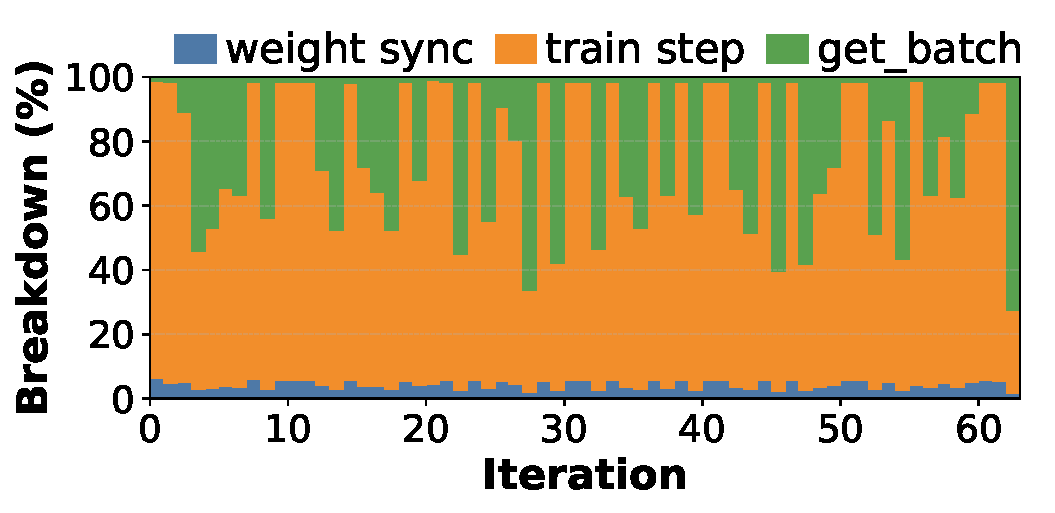
\includegraphics[width=\linewidth]{figs/trace/trace_dist.pdf}
\caption{step time 分布。}
\label{fig:trace_dist}
\end{subfigure}
\begin{subfigure}[b]{0.33\linewidth}
\centering
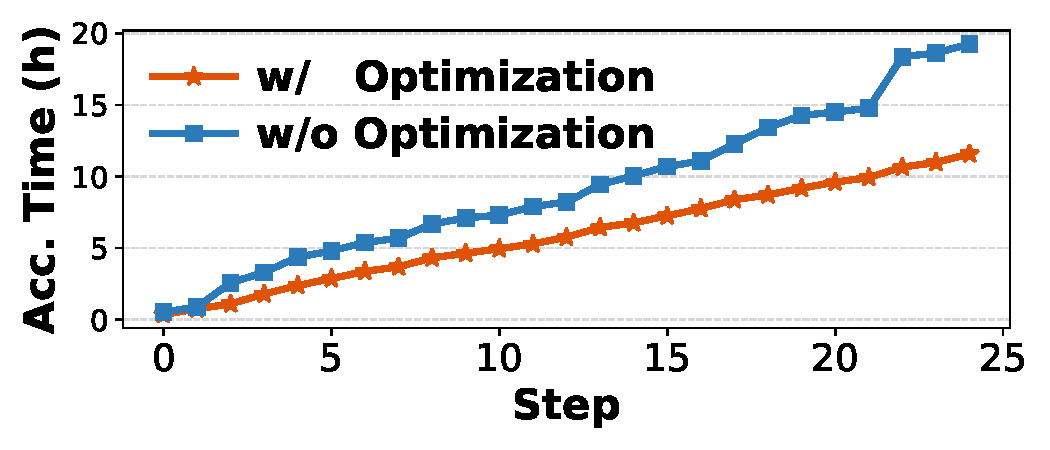
\includegraphics[width=\linewidth]{figs/trace/total_iter_time.pdf}
\caption{累计 step time。}
\label{fig:opt_step_time}
\end{subfigure}
\caption{生产级 agentic RL 工作负载画像。}
\label{fig:workload_overview}
\end{figure*}

\subsection{原则 3：Serverless 奖励工作者的收益}
\label{subsec:eval-reward-worker}
我们将 \textit{Reward-as-a-Service} 与本地专用 GPU 奖励部署做对比。在 16 卡集群上并发运行 3 个数学任务作业时，本地方案需要为奖励 LLM 预留 4 张 GPU，而 serverless 平台由 3 个作业共享并自动扩缩容。\autoref{fig:reward_comparison_exp} 显示，serverless 方案将平均 GPU 利用率从 6\% 提高到 88\%，并把单步 rollout 时间从 158 秒降到 77 秒。换言之，将无状态奖励从本地热备 GPU 中剥离出来，不仅减少资源浪费，也让更多 GPU 可以参与 rollout，从而带来显著端到端收益。
